\documentclass[spanish,12pt,a4paper,titlepage]{report}
\usepackage[utf8]{inputenc}
\usepackage{graphicx}
\usepackage{subfig}
\usepackage{float}
\usepackage{wrapfig}
\usepackage{multirow}
\usepackage{caption}
\usepackage[spanish]{babel}
\usepackage[dvips]{hyperref}
\usepackage{amssymb}
\usepackage{listings}
\usepackage{epsfig}
\usepackage{amsmath}
\usepackage{array}
\usepackage[table]{xcolor}
\usepackage{multirow}
%\usepackage[Sonny]{fncychap}
\usepackage[Lenny]{fncychap}
%\usepackage[Glenn]{fncychap}
%\usepackage[Conny]{fncychap}
%\usepackage[Rejne]{fncychap}
%\usepackage[Bjarne]{fncychap}
%\usepackage[Bjornstrup]{fncychap}

%\usepackage{subfiles}
%\usepackage{framed}

\setlength{\topmargin}{-1.5cm}
\setlength{\textheight}{25cm}
\setlength{\oddsidemargin}{0.3cm} 
\setlength{\textwidth}{15cm}
\setlength{\columnsep}{0cm}

\begin{document}

\chapter{División de tareas}

\begin{figure}[h!]
	\centering
	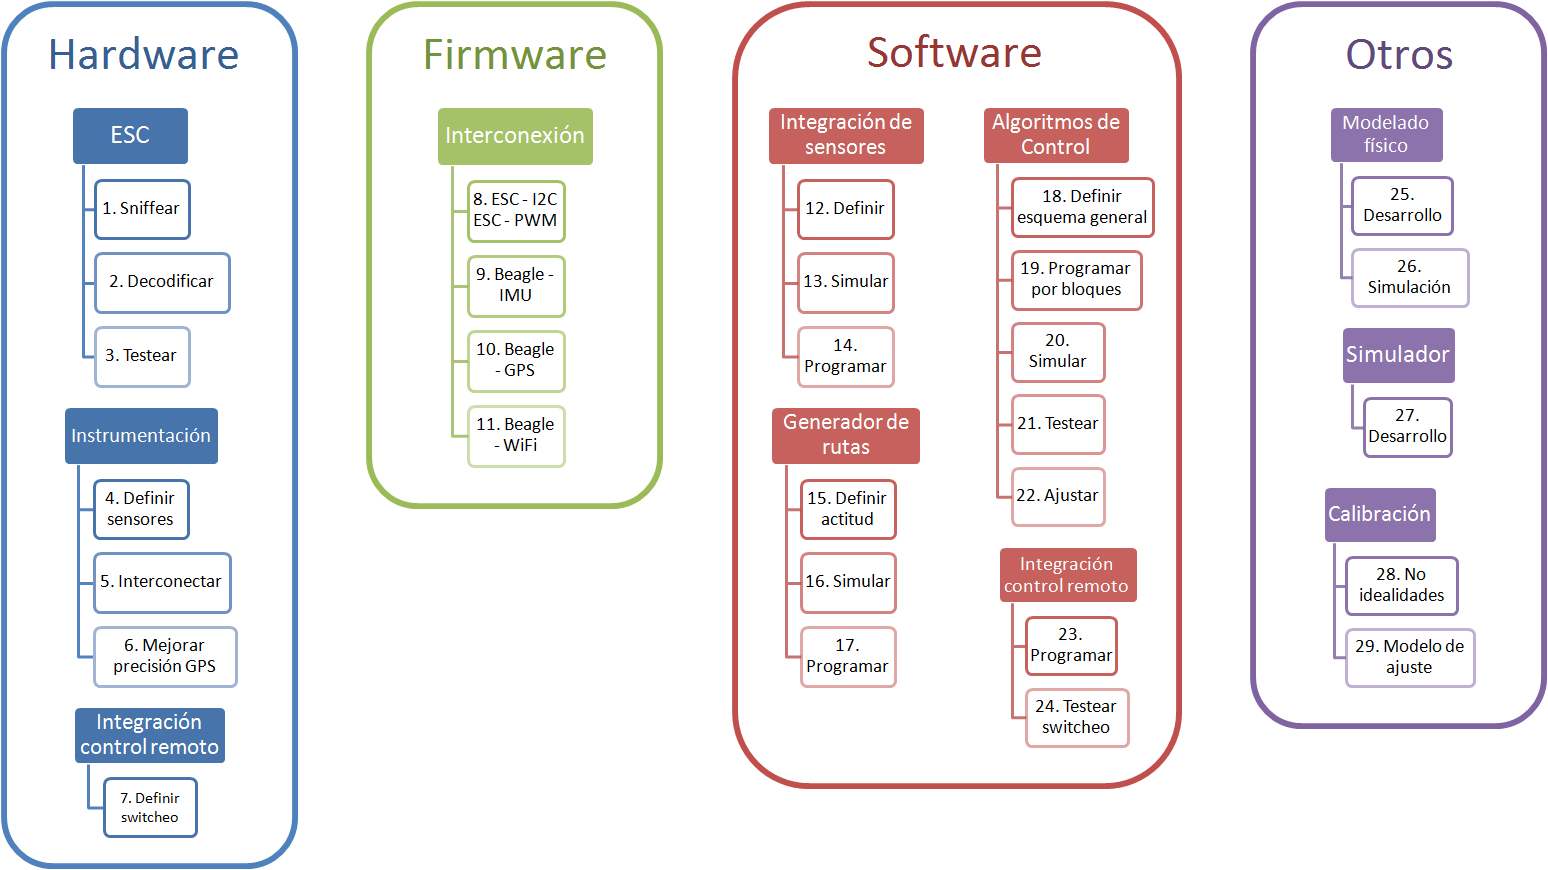
\includegraphics[width=1\textwidth]{./division.png}
	\caption{División de tareas}
	\label{fig:div}
\end{figure}

\begin{enumerate}
	\item Hacer funcionar el analizador lógico
	\item Decodificar el código I2C, entenderlo y aprender a enviar comandos
	\item Probar si los comandos enviados producen el efecto deseado sobre los motores
	\item Investigar en papers u otros documentos si será necesario incluir algún otro sensor
	\item Interconectar todos los sensores, armar los conversores de niveles lógicos necesarios
	\item Investigar e implementar alguna manera de mejorar la presición del GPS
	\item Definir la forma de realizar el switcheo entre el control remoto y el control automático. Definir el hardware necesario para ello
	\item Programar el firmware necesario para una buena comunicación entre los \textbf{ESC's} y los motores, ya sea mediante protocolo \textbf{I2C} o \textbf{PWM}
	\item Programar el firmware necesario para una buena comunicación entre la \textbf{BeagleBoard} y la \textbf{IMU}.
	\item Programar el firmware necesario para una buena comunicación entre la \textbf{BeagleBoard} y el \textbf{GPS}.
	\item Programar el firmware necesario para una buena comunicación entre la \textbf{BeagleBoard} y el dispositivo \textbf{Wi-Fi}.
	\item Definir criterios para integrar los sensores: algoritmo base, interrogación periódica a los sensores, cada cuanto tiempo, en que orden, etc.
	\item Simular los algoritmos y corroborar el buen funcionamiento teórico.
	\item Programar los algoritmos definitivos y probarlos
	\item Definir la actitud de vuelo del cuadricóptero.
	\item simular vuelo en MatLab.
	\item Programar algoritmos definitivos y testearlos.
	\item Definir el esquema general de los algoritmos de control
	\item Programar los distintos bloques de control y su interrelación
	\item Simular algoritmos de control
	\item Testear algoritmos de control
	\item Realizar los ajustes necesarios y reprogramar si es necesario
	\item Programar el software necesario para la conmutación entre el control automático y el remoto.
	\item Desarrollo del modelo físico y contrastación con papers existentes
	\item Simular el comportamiento del cuadricóptero según el modelo físico.
	\item Desarrollar el simulador en MatLab
	\item Identificar las no idealidades de los sensores
	\item Implementar un modelo de ajuste de las medidas tomadas por los sensores, diseñar pruebas y en función de estas hallar los parámetros de los modelos propuestos para finalmente calibrar de la mejor forma los sensores.
\end{enumerate}

\end{document}